%%%%%%%%%%%% struct manager configuration
\ifxHPTDC{
	\subsection{Structure \prefix manager\tu configuration}
	\cronvar{\prefix device\tu configuration}{device\tu configs[\PREFIX DEVICES\tu MAX]}\\
	A structure with the configuration for an individual \deviceName\ board as defined in the next subsection.
	Use the function \textsf{\prefix count\tu devices()} to query how many entries contain valid information. See section \ref{countdevices} for details. \par 

	\cronvar{\prefix grouping\tu configuration}{grouping}\\
	Structure with the parameters for grouping. 
	See section \ref{structgrouping} for the definition of the structure and section \ref{grouping} for more information on grouping.\par

	\cronvar{void}{*bin\tu to\tu ps}\\
	Reserved for future use.
	
}{}
%%%%%%%%%%%%%% struct device_configuration
\subsection{Structure \prefix \ifxHPTDC{device\tu}{}configuration}

	This is the structure containing the configuration information. 
	\ifxHPTDC{}{ % xHPTDC8 uses TDC manager instead
		It is used in conjunction with \textsf{\prefix get\tu default\tu configuration()}, \textsf{\prefix get\tu current\tu configuration()} and \textsf{\prefix configure()}.\par
	}
	It uses the multiple substructures to configure various aspects of the board. 

	\cronvar{int}{size}\\
	The number of bytes occupied by the structure.\par

	\cronvar{int}{version}\\
	A version number that is increased when the definition of the structure is changed. The increment can be larger than one to match driver version numbers or similar. Currently only version 0 is defined.\par

	% autotrigger was reordered for the xHPTDC so we need to be able to use it in conditionally
	\newcommand{\autotrigger}{			
		\cronvar{int}{auto\tu trigger\tu period}\\
		\cronvar{int}{auto\tu trigger\tu random\tu exponent}\\
		Create a trigger either periodically or randomly. There are two parameters $M = \text{trigger\tu period}$ and $N = \text{random\tu exponent}$ that result in a distance between triggers of $T$ clock cycles.

		\begin{align}
			T &= 1 + M + [1...2^N]\\
			&0 \leq M < 2^{32}\\
			&0 \leq N < 32
		\end{align}

		\noindent There is no enable or reset. The auto trigger is running continously. 
		The usage of this trigger can be configured in the TiGer block source field.\par
	}
	\ifxHPTDC{
		\autotrigger
	}{}

	\cronvar{int}{tdc\tu mode}\\
	\ifxHPTDC{
		This defines whether grouping is used by the \textsf{\prefix read\tu hits()} method. \\
		Defaults to continuous mode. \\*
		\begin{tabular}{lc}
			\ttdef{TDC\tu MODE\tu GROUPED} & 0   \\
			\ttdef{TDC\tu MODE\tu CONTINUOUS} & 1   \\
		\end{tabular}
	}{
		TDC mode. Can be grouped or continuous.
		Currently only \textsf{\PREFIX TDC\tu MODE\tu GROUPED} is supported. 
		This is set per default by \textsf{\prefix get\tu current\tu configuration()} and should be left unchanged.
	}\par

	\ifxHPTDC{} % does not exist for xHPTDC8
	{
		\cronvar{crono\tu bool\tu t}{start\tu rising} 
		\itett{
			Not applicable for the \deviceName.
		}{
			Selects whether the rising or falling edge of the start signal is used to start a group.
		}\par
	}

	\cronvar{double}{dc\tu offset[\PREFIX TDC\tu CHANNEL\tu COUNT + 1]}\\	
	Set the threshold voltage for the input channels \ifxHPTDC{A \ldots H and TRG}{S, A \ldots D} (see figure \ref{fig:dcoffset1}).
	\begin{itemize}
		\ifxHPTDC{
			\item dc\tu offset[0 - 7] : threshold for channels A \ldots H
			\item dc\tu offset[8] : threshold for channel TRG
		}{
			\item dc\tu offset[0] : threshold for channel Start
			\item dc\tu offset[1 - 4] : threshold for channels A \ldots D
		}
	\end{itemize}
	Supported range is -1.32V to +1.18V. This should be close to 50\% of the height of the input pulse. Examples for various signaling standards are defined as follows:\par
	\begin{tabular}{ll}
		\ttdef{DC\tu OFFSET\tu P\tu NIM} & +0.35\\
		\ttdef{DC\tu OFFSET\tu P\tu CMOS} & +1.18\\
		\ttdef{DC\tu OFFSET\tu P\tu LVCMOS\tu 33} & +1.18\\
		\ttdef{DC\tu OFFSET\tu P\tu LVCMOS\tu 25} & +1.18\\
		\ttdef{DC\tu OFFSET\tu P\tu LVCMOS\tu 18} & +0.90\\
		\ttdef{DC\tu OFFSET\tu P\tu TTL} & +1.18\\
		\ttdef{DC\tu OFFSET\tu P\tu LVTTL\tu 33} & +1.18\\
		\ttdef{DC\tu OFFSET\tu P\tu LVTTL\tu 25} & +1.18\\
		\ttdef{DC\tu OFFSET\tu P\tu SSTL\tu 3} & +1.18\\
		\ttdef{DC\tu OFFSET\tu P\tu SSTL\tu 2} & +1.18\\
		\ttdef{DC\tu OFFSET\tu N\tu NIM} & -0.35\\
		\ttdef{DC\tu OFFSET\tu N\tu CMOS} & -1.32\\
		\ttdef{DC\tu OFFSET\tu N\tu LVCMOS\tu 33} & -1.32\\
		\ttdef{DC\tu OFFSET\tu N\tu LVCMOS\tu 25} & -1.25\\
		\ttdef{DC\tu OFFSET\tu N\tu LVCMOS\tu 18} & -0.90\\
		\ttdef{DC\tu OFFSET\tu N\tu TTL} & -1.32\\
		\ttdef{DC\tu OFFSET\tu N\tu LVTTL\tu 33} & -1.32\\
		\ttdef{DC\tu OFFSET\tu N\tu LVTTL\tu 25} & -1.25\\
		\ttdef{DC\tu OFFSET\tu N\tu SSTL\tu 3} & -1.32\\
		\ttdef{DC\tu OFFSET\tu N\tu SSTL\tu 2} & -1.25\\
	\end{tabular}\par
		\noindent The inputs are AC coupled. Thus, the absolute voltage is not important for pulse inputs. 
		It is the relative pulse amplitude that causes the input circuits to switch. \textit{dc\tu offset} must be set to the relative switching voltage for the input standard in use. If the pulses are negative, a negative switching threshold must be set and vice versa.
	\begin{figure}
		\begin{center}
			\ifxHPTDC{
				\includegraphics[width=0.3\textwidth]{xhptdc/figures/InputCircuit.pdf}
			}{
				\includegraphics[width=0.3\textwidth]{figures/InputCircuit.pdf}
			}
			\caption{Input circuit for each of the input channels. \label{fig:dcoffset1}}
		\end{center} 
	\end{figure}
%%			\begin{figure}
%%				\begin{center}
%%					\includegraphics[width=\textwidth]{figures/dc_offset.pdf}
%%%					\caption{\textit{dc\tu offset} is used to shift the signal on each input channel such that the noise margin relative to the switching threshold is maximized.
%%					Insets of figure a) and b) show the base line of the signal with $\mathrm{\textit{dc\tu offset}}~=~0$ close to the switching threshold of the input buffer. Figure a) shows the positive pulse with $\mathrm{\textit{dc\tu offset}}~>~0$ and figure b) shows the negative pulse with $\mathrm{\textit{dc\tu offset}}~<~0$.\label{fig:dcoffset2}}
%%				\end{center}
%%			\end{figure}

	\ttvar{\prefix trigger}{trigger[\PREFIX TRIGGER\tu COUNT]}\\
	Configures the polarity of the external trigger sources.
	These are used as inputs for the TiGer blocks and as inputs to the time measurement unit.\par

	\ttvar{\prefix tiger\tu block}{tiger\tu block[\PREFIX TIGER\tu COUNT]}\\
	Configuration of the timing generators (TiGer).

	\ifxHPTDC{
		\ttvar{\prefix tiger\tu block}{gating\tu block[\PREFIX GATE\tu COUNT]}\\
		Configuration of the gating blocks.	
	}{} % only for xHPTDC8

	\ttvar{\prefix channel}{channel[\PREFIX CHANNEL\tu COUNT]}\\
		Configure the TDC channels.

	\ifxHPTDC{
		\cronvar{crono\tu bool\tu t}{skip\tu alignment}\\
		If set,  the phase of the two TDC chips is not realigned when capturing is restartet.

		\cronvar{crono\tu bool\tu t}{alignment\tu source}\\
		Define a signal source that is used for phase alignment. Should usually be left unchanged.
		\begin{tabular}{ll}
			\ttdef{ALIGN\tu TIGER} & 0\\
			\ttdef{ALIGN\tu PIN} & 1\\
			\ttdef{ALIGN\tu RESERVED} & 2\\
		\end{tabular}\par
		
	}{
		\ttvar{\prefix low-res\tu channel}{low-res\tu channel[\PREFIX LOWRES\tu CHANNEL\tu COUNT]}\\
		\itett{
			Not applicable for \deviceName. 
		}{
			Only applicable to the xTDC4-Sciex. Configures the additional digital low-res inputs.
		}\par
		\autotrigger
	
	}

	

%%%%%%%%% trigger
	\subsection{Structure \prefix trigger}
	\label{structtrigger}
	For each input this structure determines wheter rising or falling edges on the inputs create trigger events for the TiGer \ifxHPTDC{and gating}{} blocks.

	\cronvar{crono\tu bool\tu t}{falling}\\
	\cronvar{crono\tu bool\tu t}{rising}\\
	Select for which edges a trigger event is created inside the FPGA.
	\txh{
		Set the corresponding flag for one of the edges or both edges then using the input with a TiGer.
	}{
		The \deviceName can output measurements with a reduced bin size of $5/6~ns = 833,\overline{3}~ps$ for one or both edges of input signals. 
		See section \ref{difficulthits} for more information on hits with varying resolution.
		Use \textsf{xtdc4\tu channel.rising} on page \pageref{structchannel} to select which edge is measured with full resolution.
		The edge that is selected for full resolution measurement must also be enabled for low resolution measurement.
	}{
		While the TDC can only measure either rising or falling edges, the gating blocks and the TiGer are more flexibel. 
		Set the corresponding flag for one of the edges or both edges when using the input with a TiGer or gating block.
	}\par

%%%%% tiger_block			

	\subsection{Structure \prefix tiger\tu block\label{cp:tigerblock}}
	See section \ref{cp:tiger} for additional information.
	\ifxHPTDC{
		\cronvar{int}{mode}\\*
		Enables the desired mode of operation for the tiger. \\*
		\begin{tabular}{lrl}
			\ttdef{TIGER \tu OFF} & 0 & No operation \\
			\ttdef{TIGER \tu OUTPUT} & 1 & Output is driven with 2V amplitude. \\*
										&   &There must be no input connected \\
			\ttdef{TIGER \tu BIDI} & 2 & Output is driven with 1V amplitude. \\*
									&   & Pulse rate should be low. \\*
			\ttdef{TIGER \tu BIPOLAR} & 3 & Output is driven with 1~V bidirectional pulses.\\*
									&   & $start = stop -1$\\*
		\end{tabular}
		The gating blocks are only used internally and produce no pulses accessible to the user.		
		Gating blocks interpret any value that is not 0 as as enable.\\*
		\begin{tabular}{lrl}
			\ttdef{GATE \tu OFF} & 0 & No gating, alle hits are captured. \\*
			\ttdef{GATE \tu ON} & 1 & No hits are captured while the gate is active.\\*
		\end{tabular}
	
	}{
		\cronvar{crono\tu bool\tu t}{enable}\\
		Activates the timing generator (TiGer).\par
	}

	\cronvar{crono\tu bool\tu t}{negate}\\
	Inverts output polarity. Default is set to false.
	\ifxHPTDC{For gating blocks, a value of false blocks inputs between start and stop, a value of true blocks outputs outside that interval.
	The TiGer creates a high pulse from \textsf{start} to \textsf{stop} unless negated.}{}\par

	\cronvar{crono\tu bool\tu t}{retrigger}\\
	Enables retrigger setting.\\
	If enabled the timer is reset to the value of the \textsf{start} parameter, whenever the input signal is set while waiting to reach the \textsf{stop} time.\par

	\cronvar{crono\tu bool\tu t}{extend}\\
	Not implemented.

	\ifxHPTDC{}{
		\cronvar{crono\tu bool\tu t}{enable\tu lemo\tu output}\\
		Enables the LEMO output. Drive the TiGer Signal to the corresponding Lemo connector as an output. 
		This is DC coupled, so make sure that you do not any devices connected as inputs.
		Pulses created by the TiGer are visible at the \deviceName inputs and can be measured again to get the exact timing.  
	}

	\cronvar{int}{start}\\
	\cronvar{int}{stop}\\
	\itett{
		In multiples of $4~ns$.
	}{
		In multiples of $20~ns/3 = 6,\overline{6}~ns$
	}
	The time during which the TiGer output is set, relative to the trigger input. The parameters \textsf{start} and \textsf{stop} must fulfill the following conditions:
	\[ 0 <= start <= stop <= 2^{16}-1 \]
	If retriggering is enabled, the timer is reset to the value of the start parameter whenever the input signal is set while waiting for the stop time. \par
	

	\cronvar{int}{sources}\\
	A bit mask with a bit set for all trigger sources that can trigger this TiGer block. 
	Default is \textsf{\PREFIX TRIGGER\tu SOURCE\tu \ifxHPTDC{A}{S}}.\par

	\begin{tabular}{lc}
			\ttdef{TRIGGER\tu SOURCE\tu NONE} & 0x00000000\\
		\ifxHPTDC{
			\ttdef{TRIGGER\tu SOURCE\tu A} & 0x00000001\\
			\ttdef{TRIGGER\tu SOURCE\tu B} & 0x00000002\\
			\ttdef{TRIGGER\tu SOURCE\tu C} & 0x00000004\\
			\ttdef{TRIGGER\tu SOURCE\tu D} & 0x00000008\\
			\ttdef{TRIGGER\tu SOURCE\tu E} & 0x00000010\\
			\ttdef{TRIGGER\tu SOURCE\tu F} & 0x00000020\\
			\ttdef{TRIGGER\tu SOURCE\tu G} & 0x00000040\\
			\ttdef{TRIGGER\tu SOURCE\tu H} & 0x00000080\\
			\ttdef{TRIGGER\tu SOURCE\tu TDC1\tu SYNC} & 0x00000100\\
			\ttdef{TRIGGER\tu SOURCE\tu TDC2\tu SYNC} & 0x00000200\\
			\ttdef{TRIGGER\tu SOURCE\tu TDC\tu EXT\tu SYNC} & 0x00000400\\
			\ttdef{TRIGGER\tu SOURCE\tu ADC1\tu CONV} & 0x00000800\\
			\ttdef{TRIGGER\tu SOURCE\tu ADC2\tu CONV} & 0x00001000\\
			\ttdef{TRIGGER\tu SOURCE\tu AUTO} & 0x00004000\\
			\ttdef{TRIGGER\tu SOURCE\tu ONE}  & 0x00008000	
		}{
				\ttdef{TRIGGER\tu SOURCE\tu S} & 0x00000001\\
				\ttdef{TRIGGER\tu SOURCE\tu A} & 0x00000002\\
				\ttdef{TRIGGER\tu SOURCE\tu B} & 0x00000004\\
				\ttdef{TRIGGER\tu SOURCE\tu C} & 0x00000008\\
				\ttdef{TRIGGER\tu SOURCE\tu D} & 0x00000010\\
				\ttdef{TRIGGER\tu SOURCE\tu AUTO} & 0x00004000\\
				\ttdef{TRIGGER\tu SOURCE\tu ONE} & 0x00008000
		}
	\end{tabular} 

%%%%%%%%%%%%%%%%%%%%%%%% channel

	\subsection{Structure \prefix channel}
		\label{structchannel}
		Contains TDC channel settings.\par

		\cronvar{crono\tu bool\tu t}{enable\ifxHPTDC{}{d}}\\
		Enable TDC channel.\par

		\cronvar{crono\tu bool\tu t}{rising}\\
		\txh{
			Not applicable for \deviceName.
		}{
			Select which edge of the signal is used for full resolution measurements. 
			\textsf{xtdc4\tu trigger.rising} and \textsf{xtdc4\tu trigger.falling} described on page \pageref{structtrigger} are used 
			to select which edges are recorded for low resolution measurement. 
			The edge that is selected for full resolution measurement must also be enabled for low resolution measurement.
			See section \ref{difficulthits} for more information on hits with varying resolution.
		}{
			Select which edge of the signal is measured by the TDC. 
			The TiGer and gating blocks use a separate configuration that allows to use both edges simultaneously on each input. See section \ref{structtrigger}
		}\par

		\txh{}{ %only for xTDC4
			\cronvar{crono\tu bool\tu t}{cc\tu enable}\\
			Enable carry chain TDC. This is set to \emph{true} by default and should be left unchanged. \par

			\cronvar{crono\tu bool\tu t}{cc\tu same\tu edge}\\
			Sets whether the carry chain TDC records the same or opposite edge as the TDC chip. 
			If the same edge is selected, that carry chain TDC acts  as a backup if the chip misses hits due to FIFO overflows or short input pulses.
			If opposite edges are selected, both edges of a pulse can be measured with reasonable resolution. See section \ref{difficulthits} for more information.\par

			\cronvar{crono\tu bool\tu t}{ths788\tu disable}\\
			Disable full resolution timestamps. This is set to \emph{false} by default and should be left unchanged.\par
		}{}

		\ifxHPTDC{}{
			\cronvar{int}{start}\\
			\cronvar{int}{stop}\\
			Veto function for grouping of hits into packets in multiples of the binsize. Only hits between start and stop are read out.
			The parameters must adhere to the following relations:
			\[
				0 <= start <= stop < 2^{ \itett{31}{30}}
			\]
		}

%%%%%%%%%%%%%%%%%%%%% grouping, only fpr xHPTDC8

\ifxHPTDC{
	\subsection{Structure \prefix grouping\tu configuration}	
	\label{structgrouping}
	This structure configures the behaviour of the grouping functionality. See section \ref{grouping}.
	Grouping is enabled with the \textsf{tdc\tu mode} paramter defined in the top level of the config structure.

	In this structure intervals are always provided in picoseconds, independently of the bin size of the TDC.

	\cronvar{int}{trigger\tu channel}\\
	Channel number that is used to trigger the creation of a group.\par

	\cronvar{int}{zero\tu channel}\\
	Optionally a different channel can be used to calculate the relative timestamps in a group. 
	This is disabled per default by setting this paramteer to $-1$.\par
	
	\cronvar{\tu\tu int64}{zero\tu channel\tu offset}\\
	This offset in picoseconds is added to relative timestamps within a group.\par

	\cronvar{\tu\tu int64}{range\tu start}\\
	\cronvar{\tu\tu int64}{range\tu stop}\\
	Values in the interval from \textsf{range\tu start} to \textsf{range\tu stop} are included in the group. 
	Either or both values can be negative to create common-stop behaviour. 
	\[
		-2^{63} \le range\_start \le range\_stop < 2^{63} 
	\]\par

	\cronvar{\tu\tu int64}{trigger\tu deadtime}\\
	After a trigger was detected additional triggers will be suppressed for this interval. Must not be negative.\par

	\cronvar{crono\tu bool\tu t}{require\tu windows\tu hit}\\
	If set a group is only created if there is at least one hit in the window defined by \textsf{window\tu start} and \textsf{window\tu stop}.\par

	\cronvar{\tu\tu int64}{window\tu start}\\
	\cronvar{\tu\tu int64}{window\tu stop}\\
	\[
		-2^{63} \le window\_ start \le window\_ stop < 2^{63} 
	\]\par

	\cronvar{int}{veto\tu mode}\\
	A window defined by \textsf{veto\tu start} and \textsf{veto\tu stop} can be used to suppress hits. 
	The functionality is very similar to the gating blocks but is defined in software. 
	While gating blocks can only work locally on the information available within each board the veto function is applied globally accross all boards.
	This feature can not be used to improve FIFO usage or PCIe bandwidth usage. 
	 \\*
	Either data inside or outside the veto window can be suppressed.\\*
	\begin{tabular}{lc}
		\ttdef{VETO\tu OFF}     & 0 \\
		\ttdef{VETO\tu INSIDE}  & 1 \\
		\ttdef{VETO\tu OUTSIDE} & 2 \\
	\end{tabular}\par

	\cronvar{\tu\tu int64}{veto\tu start}\\
	\cronvar{\tu\tu int64}{veto\tu stop}\\
	\[
		-2^{63} \le veto\_ start \le veto\_ stop < 2^{63} 
	\]\par

	\cronvar{crono\tu bool\tu t}{veto\tu relative\tu zero}\\
	If set, the veto window is defined relative to the zero channel. Otherwise the window is defined relative to the trigger.\par 

	\cronvar{crono\tu bool\tu t}{overlap}\\
	Unsupported, must remain \textsf{false}.

}{}